% 2008 年江西卷文科第 22 题：抛物线 y=x^2 与三点 M(x0,y0)、P(0,y0)、N(-x0,y0)；
%   过 M 的直线交抛物线于 A、B，AP、BP 的延长线交抛物线于 E、F。
% 来源 PDF：gaokaomath-src/普通高考/2008/2008江西文.pdf
% SHA-256：8505b08b95152dbb1421e3f2d72c379b24c8ab6cb47bcc1dbdc8feb058459cda
% 原页：2008江西文.pdf 第 2 页（A3 三栏）第 3 栏，书页码 462。
% 绘制依据：按原页：抛物线开口向上，A 在左上、B 在右、M 在 B 上方偏右、P 在 y 轴上、
%   N 在 y 轴左侧；A—M—B 为割线，A—P—E 与 B—P—F 为两条直线，N—F—E—M 虚线为共线迹。
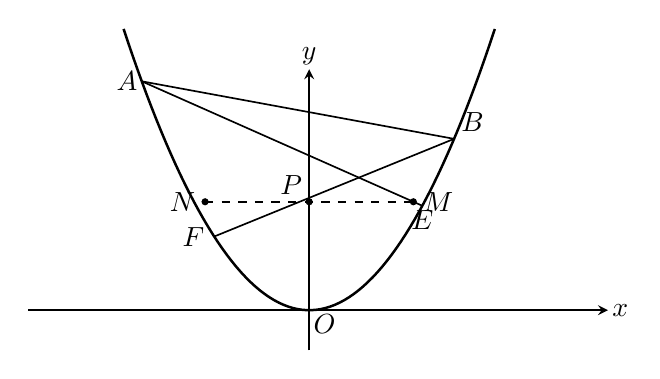
\begin{tikzpicture}[x=1.15cm, y=0.85cm, semithick, every node/.style={inner sep=1.3pt}]
  \draw[->,>=stealth] (-3.1,0) -- (3.3,0) node[right] {$x$};
  \draw[->,>=stealth] (0,-0.6) -- (0,3.6) node[above] {$y$};
  \node[below right] at (0,0) {$O$};

  \draw[line width=0.9pt, domain=-2.05:2.05, samples=80] plot (\x, {\x*\x});

  \coordinate (A) at (-1.85,3.42);
  \coordinate (M) at (1.15,1.62);
  \coordinate (B) at (1.60,2.56);
  \coordinate (P) at (0,1.62);
  \coordinate (N) at (-1.15,1.62);
  \coordinate (E) at (1.25,1.56);
  \coordinate (F) at (-1.05,1.10);

  \draw (A) -- (B);
  \draw (A) -- (E);
  \draw (B) -- (F);
  \draw[dashed] (N) -- (M);

  \fill (P) circle (1.3pt);
  \fill (M) circle (1.3pt);
  \fill (N) circle (1.3pt);

  \node[left] at (A) {$A$};
  \node[above right=1pt] at (B) {$B$};
  \node[right=2pt] at (M) {$M$};
  \node[above left=1pt] at (P) {$P$};
  \node[left=2pt] at (N) {$N$};
  \node[below] at (E) {$E$};
  \node[left=2pt] at (F) {$F$};
\end{tikzpicture}
